%%%%%%%%%%%%%%%%%%%%%%%%%%%%%%%
% Mathiesen/Evrard Test Paper %
%%%%%%%%%%%%%%%%%%%%%%%%%%%%%%%

%%%%%%%%%%
% Header %
%%%%%%%%%%
\documentclass[12pt, preprint]{aastex}
%\documentclass{emulateapj}
%\usepackage{graphicx}
\usepackage{here,lscape}
\newcommand{\myemail}{astrosriram@yahoo.co.in}
\newcommand{\grs}{GRS~1915+105}
\newcommand{\x}{Cygnus~X-3}
\newcommand{\Au}{4U~1630-47}
\newcommand{\xtj}{XTE~J1550-564}
%\begin{center}
%{\large\bf Introduction}
%\end{center}
\shorttitle{Mathiesen-Evrard Test}
\shortauthors{Cavagnolo et al.}
\bibliographystyle{apj}

%%%%%%%%%%%%%%%%%%%%%
% Title and Authors %
%%%%%%%%%%%%%%%%%%%%%

\begin{document}
\title{Detection of Hierarchical Structure Formation\\
       Using Mathiesen-Evrard Test}
\author{Kenneth Cavagnolo\altaffilmark{1,2}, Megan Donahue\altaffilmark{1}, Mark Voit\altaffilmark{1}, and Ming Sun\altaffilmark{1}}
\altaffiltext{1}{Department of Physics and Astronomy, Michigan State University, BPS Building, East Lansing, MI 48824}
\altaffiltext{2}{cavagnolo@pa.msu.edu}

%%%%%%%%%%%%
% Abstract %
%%%%%%%%%%%%

\begin{abstract}
We present spectral analysis for an {/textit{Chandra}} Archival sample of 169 X-Ray
luminous clusters of galaxies. We measure and compare temperatures for
the [0.7-7.0]keV and [2.0/(1+z)-7.0]keV bandpasses. Defining
T$_{frac}$ as T$_{[0.7-7.0]}/$T$_{[2.0-7.0]}$, we find T$_{frac}
\gtrsim$ 1 for 149 clusters of which 73 are significant at the 90\%
confidence level. The clusters with the highest T$_{frac}$ are the most massive, typically are
lensers, and undergoing major mergers. We suggest T$_{frac}$ as a spectroscopic
tracer of structure formation that can be utilized in simulations to
track the degree of virialization.
\end{abstract}

%%%%%%%%%%%%
% Keywords %
%%%%%%%%%%%%

\keywords{catalogs -- galaxies: clusters: general -- X-rays:
  galaxies: clusters -- cosmology: observations -- methods: data
  analysis}

%%%%%%%%%%%%%%%%%%%%%%%%%%%%%%%%%%%%%%%
\section{Introduction}\label{sec:intro}
%%%%%%%%%%%%%%%%%%%%%%%%%%%%%%%%%%%%%%%

The X-Ray properties of a cluster of galaxies are a fundamental tool
for understanding the evolution, radiative cooling, and
feedback mechanisms which define global cluster
properties such as temperature, pressure, and entropy
distributions. Accurate measurement of these cluster properties influences the
determination and interpretation of cluster masses and their subsequent use in
studies of cosmological models via assumption of hydrostatic
equilibrium and use of the mass-temperature relation
(\cite{2005RvMP...77..207V},
\cite{1996ApJ...469..494E}). The accuracy of simulations to replicate
these observational properties will further our understanding of how
clusters came to look the way they do at present, and ultimately the
exact values for the cosmological model defining our Universe.

To this end, X-Ray spectroscopic study of the intracluster medium
(ICM) tells us about the temperature and gas density distribution in a
cluster and thus the mass distribution. It is often assumed however
that multiphase plasma
arising from gas inhomogeneities like shocks, cold fronts, radio lobes, and/or
filaments, when integrated within an aperture, yields a single
temperature which is representative of
the global cluster properties within the aperture and the underlying
physics thereof. This may not
always be the case though as there are many observational systematics
which influence the accuracy of such a measurement. The ensemble of
cluster simulations originally carried out by \cite{2001ApJ...546..100M}
(hereafter ME01) found the spectroscopic temperatures, T$_{Spec}$, calculated for their
simulated clusters underestimated the mass-weighted, T$_M$, or
emission-weighted, T$_E$, temperatures by upwards of 20\%. This result was later
reproduced by several other groups using their own sets of simulations,
\cite{2004MNRAS.354...10M} (MZ04),
\cite{2004MNRAS.351..505G} (GI04), \cite{2006MNRAS.369.2013R} (RA06), and
\cite{2006astro.ph.11018K} (KA06). These temperature measures vary based on
the weighting function, $W$, used to calculate projected temperature,

\begin{equation}
T_{proj} = \frac{\int W T_{gas} dV}{\int W dV}
\end{equation}

where T$_{proj}$ is projected temperature an observer would measure,
T$_{gas}$ is the true temperature of the gas, and $W$ takes on the
mass of the gas particle, $m$, in the mass-weighted
case or the cooling function times the gas density squared,
$\Lambda(T)\rho^2$, for the emission-weighted case
(\cite{1995MNRAS.275..720N}). ME01 used the special
case of emission-measure weighting, $\Lambda(T)=1$, in their
calculation of T$_E$ while MZ04, GI04, RA06, and KA06 use variants of
the bolometric cooling function
$\Lambda(T)=\int_{0}^{\infty}\epsilon_E dE$
(\cite{1993ApJS...88..253S}). Both forms of the cooling function
assume the dominant emission from the gas is bremsstrahlung,
or free-free electron radiation. However, there is also significant
line emission from the low temperature (T $\lesssim 3$keV) gas in
clusters which drives the integrated temperature lower than would be
expected from pure bremsstrahlung emission. ME01 state the
underprediction of T$_E$ and T$_M$ is the result of cool subclumps
accreting into the cluster which introduces an excess in the soft
X-Rays and is not spectroscopically resolvable. The consequence of
this bias is an underprediction of cluster binding masses by $15-30\%$.

ME01 propose an observational test for this effect using the
{\textit{Chandra}} telescope. They suggest using the photons from the
$[0.5-9.5]$keV band (which will include the line and bremsstrahlung
emission from the cluster) and the $[2.0-9.5]$keV band (which will only
include the bremsstrahlung emission) as a diagnostic for measuring the
bias created from the prescence of unresolved cool gas. The predicted
mathematical form of this bias is

\begin{equation}
kT_{[0.5-9.5]keV} = (0.81\pm0.01)kT_{[2.0-9.5]keV}^{1.09\pm0.01}.
\end{equation}

The focus of this paper is to observationally test for such a bias
using real observations taken with the {\textit{Chandra}} telescope.
Using two separate energy bandpasses we seek to remove or
constrain all possible systematics from the data analysis and
then look for either the prescence or abscence of this bias. MZ04
and \cite{2006ApJ...640..710V} have derived algorithms for calculating
the ``proper'' spectroscopic temperature for two-phase gas where one
component is unresolved cool gas at T$\gtrsim 3.0$keV and T$\gtrsim
0.5$keV, respectively.

%% Do we find observational motivation to calculate T_proper from
%% T_Spec across the board, or is this only a useful device within a
%% particular temperature range?
%% Mention the sim'd spectra useage for constraining the observational
%% limits of this bias.

This paper proceeds in the following manner. In \S\ref{sec:selection}
we outline the criteria and subsequent {\textit{Chandra}} observations selected for
study. Data reduction and handling of the X-Ray background is
discussed in \S\ref{sec:data}. Spectral extraction, fitting, and systematics are
discussed in \S\ref{sec:extraction} and \S\ref{sec:fitting}. We investigate the constraints of physical
properties for cooler, unresolved components in
\S\ref{sec:simulated}. Discussion of our results are found in
\S\ref{sec:discussion}. A final summary of our work is
presented in \S\ref{sec:summary}.

%%%%%%%%%%%%%%%%%%%%%%%%%%%%%%%%%%%%%%%%%%%%%%%%
\section{Sample Selection} \label{sec:selection}
%%%%%%%%%%%%%%%%%%%%%%%%%%%%%%%%%%%%%%%%%%%%%%%%

% RBC flux-limited to 4.4x10^-12 ergs cm^-2 s^-1 in 0.1-2.4keV, z<0.3
% RBC flux-limited to 2.8x10^-12 ergs cm^-2 s^-1 in 0.1-2.4keV, z<0.41
% B55 sample flux-limited to 1.7x10^-11 ergs cm^-2 s^-1, z<0.15

Our sample comes exclusively from the {\textit{Chandra}} X-Ray
Telescope's Data Archive (CDA). We initially drew our sample from the
{\textit{ROSAT}} Brightest Cluster Sample (RBC,
\cite{1998MNRAS.301..881E}), RBC Extended Sample (RBCE,
\cite{2000MNRAS.318..333E}), and {\textit{ROSAT}} Brightest 55 Sample
(B55, \cite{1990MNRAS.245..559E}, \cite{1998MNRAS.298..416P}). While
these samples provide a complete, flux-limited sample down to
$1.7\times10^{-11}$ ergs cm$^{-2}$ sec$^{-1}$, the volume-limit of each
sample is not as deep as we desire (RBC z $\leq 0.3$, RBCE z
$\leq 0.41$ and B55 z $\leq 0.15$) to explore a broad dynamical
range. Thus we incorporated clusters from the CDA at a redshift large enough
to where a minimum of $r_{2500}$ ($r_{\Delta_c}$ being the radius at which the
average cluster density is $\Delta_c$ times the critical density of the
Universe, $\rho_c$) is within the Chandra ACIS-S or ACIS-I field of
view. The portion of our sample at z $\gtrsim 0.4$ can also be found in a
combination of the {\textit{Einstein}} Extended Medium Sensitivity Survey
(\cite{1990ApJS...72..567G}), North Ecliptic Pole Survey
(\cite{2006ApJS..162..304H}), {\textit{ROSAT}} Deep Cluster Survey
(\cite{1995ApJ...445L..11R}), and {\textit{ROSAT}} Serendipitous Survey
(\cite{1998ApJ...502..558V}).

The result of our CDA search is a total of 230 observations of which
177 are used in this paper. The bolometric luminosities
for our sample clusters plotted as a function of
redshift are shown in Figure \ref{fig:lx_z}. Luminosities
were estimated using $r_{2500}$ (discussed in \S\ref{sec:extraction})
and a dummy response covering the energy range [0.01-100]keV. These L$_bol$ values
should be considered as lower limits given the limited field of view
used for calculation and the uncertainties introduced by using an idealized
instrument response which extends well below and above the energy
range of {\textit{Chandra}}.

Basic properties of our sample are listed in Table \ref{tab:sample}. The X-Ray
temperature and metallicity listed are taken from the Ph.D. thesis of
Don Horner\footnote{D. Horner's catalog and Ph.D. thesis are on-line at
http://asd.gsfc.nasa.gov/Donald.Horner/thesis.html}. For clusters not
observed with {\textit{ASCA}} and thus not listed in Horner's thesis,
we used a literature search to locate values. If there were no
published values for a cluster, we approximated a temperature (for the sole purpose of
computing extraction regions as is discussed in \S\ref{sec:extraction})
by recursively extracting a spectrum in the region $0.1-0.2r_{500}$
(based upon an initial guess of T$_{X}$), fitting a temperature, and
recalculating $r_{500}$. This process was repeated until a convergant
temperature was reached. This method of temperature determination has
been employed in other studies, see \cite{2006MNRAS.tmp.1068S} and
\cite{2006ApJS..162..304H} as examples.

%%%%%%%%%%%%%%%%%%%%%%%%%%%%%%%%%%%%%%%%%%%%%%%%
\section{\textit{Chandra} Data}\label{sec:data}
%%%%%%%%%%%%%%%%%%%%%%%%%%%%%%%%%%%%%%%%%%%%%%%%

%%%%%%%%%%%%%%%%%%%%
%%% NB, Aug 22nd %%%
%%% software ver %%%
%%% CIAO 3.3.0.1 %%%
%%% CALDB 3.2.2  %%%
%%%%%%%%%%%%%%%%%%%%

The simulations of ME01 and MZ04 used the energy range $[0.3-10.0]$keV
for their spectral analyses, but to make a reliable comparison with
{\textit{Chandra}} data we restrict our study focus to the spectral properties of
clusters in the energy bands $[0.7-7.0]$keV and
$[2.0/(1+z)-7.0]$keV. We exclude data below $0.7$keV to avoid the
effective area and quantum efficiency variations of the ACIS detectors, and
also exclude energies above $7.0$keV where diffuse emission is
dominated by background and the effective area is small. The spectoscopic, emission measure, and
emission-weighted measure temperatures of the simulated
clusters from ME01 and MZ04 were calculated beginning at $0.3$ keV and
$2.0$keV in the cluster rest frame, hence in our study we focus on the observational
rest frame energy $2.0/(1+z)$keV where the factor $1+z$ is due
to cosmological redshift. We began our work by deploying a robust
pipeline to reprocess the raw, primary data products for each
observation downloaded from the CDA.

%%%%%%%%%%%%%%%%%%%%%%%%%%%%%%%%%%%%%%%%%%%%%%%%%%%%%%%%%%%%%%%
\subsection{Reprocessing and Reduction}\label{sec:reprocessing}
%%%%%%%%%%%%%%%%%%%%%%%%%%%%%%%%%%%%%%%%%%%%%%%%%%%%%%%%%%%%%%%

% Do I need exposure maps for this work???

To take advantage of the latest calibrations offered by the Chandra
X-Ray Center (CXC), all data was run through our pipeline which
utilizes the suite of tools offered in the Chandra Interactive
Analysis of Observations package ({\tt CIAO}. Using {\tt CIAO
v3.3.0.1} and {\tt CALDB v3.2.2}, standard data
analysis was followed for each cluster to apply the most up-to-date
time-dependent gain correction (for re-calibration of photon energies)
and/or charge transfer inefficiency (CTI) correction (when
appropriate)(\cite{2000ApJ...534L.139T}). Observations taken in {\tt VFAINT}
mode had possible background events flagged using the {\tt check\_vf\_pha}
mode switch in {\tt acis\_process\_events}. This switch sets the detection
island to a 5x5 pixel area instead of the default 3x3 area which can
be too small to effectively flag CCD detections as the tailend
of a larger cosmic ray event .

The events list for each observation was then filtered for bad
grades and only events recorded during the good time intervals (GTI)
for chips which were live during the observation were used. For
observations taken prior to standard data processing version (SDP)
7.4, we flagged, inspected, and then removed the afterglow correction
applied as part of the older SDP pipeline. Subsequently, for observations taken
prior to SDP 7.4 in {\tt FAINT} mode or SPD 7.6 and {\tt VFAINT} mode a new
bad pixel file was constructed from the level-0 data products.

To detect and remove point sources we used the {\tt CIAO} tool {\tt
wavdetect} (\cite{2002ApJS..138..185F}), on events files filtered in
the energy range $[0.3-9.0]$keV. This energy
window extends below and above the energy range of
interest for our spectral extraction because the photons below $0.7$keV
and above $7.0$keV, while useless for diffuse emission studies, are a
good diagnostic for detecting point sources
(\cite{2000SPIE.4012...17J}). We created a mask for these
sources using $2\sigma$ ellipses as calculated from
{\tt wavdetect} based on the distribution of pixels for the point
source. Each mask was then visually inspected for spurious
detections or undetected sources. Corresponding mask regions were
ignored or added, depending on circumstance. The
mask is then applied to the observation events list, resulting in a point
source cleaned level-2 events file.

Light curve analysis was then performed using Maxim Markevitch's
contributed {\tt CIAO} script {\tt lc\_clean.sl}\footnote{Available at
http://cxc.harvard.edu/contrib/maxim/acisbg/} to check for
contamination from background flares or periods of excessively high
background. Periods with count rates $\geq 3\sigma$
and/or a factor $\geq 1.2$ of the mean background level of the
observation were removed. As prescribed by Markevitch's
cookbook\footnote{http://cxc.harvard.edu/contrib/maxim/acisbg/COOKBOOK}
ACIS front-illuminated chips were analyzed in the $[0.3-12.0]$keV range
with time bins of $259.28$ in length, and for the ACIS back-illuminated
chips, $[2.5-7.0]$keV energy range with time bins of $1037.12$ in
length. For time intervals which exhibited high background, a new GTI
file was constructed which did not include the bad epoch(s) and the
events list for each observation was again filtered.

The flare cleaned, point source excluded level-2 events file was then
centroided to determine the cluster ``center''. The determination of
the center is done using photons in the $[0.7-7.0]$keV range. Our sample includes
nearly equal numbers of clusters which appear relaxed and spherically
symmetric to clusters which have complex emission morphologies. For
clusters which appear relaxed and symmetrical, the X-Ray peak is
nearly coincident with the emission centroid and the peak is used as the
center to cut-down on unnecessary computation time. For clusters with
noticeable sub-structure, the X-Ray emission peak and emission
centroid are not coincident and thus the centroid must be calculated
and used as the center.

%%%%%%%%%%%%%%%%%%%%%%%%%%%%%%%%%%%%%%%%%%%%%%%%%%%%
\subsection{X-Ray Background} \label{sec:background}
%%%%%%%%%%%%%%%%%%%%%%%%%%%%%%%%%%%%%%%%%%%%%%%%%%%%

Because we are examining the global temperature of clusters and
specifically looking for a skewing in temperatures for energy bands
which can be extremely contaminated by the high energy particle
background or the soft local background, it was very important for
this study that we carefully analyze the background and subtract it
from our resulting spectra.

For clusters which nearly fill the field of view on
either the ACIS-S or ACIS-I detectors, diffuse emission can contaminate
any attempt at examining the local background on either CCD array. For clusters which do
not fill the field of view, utilizing a local background assumes there
is no contamination from projected cluster diffuse emission or unresolved
point sources. Our avoidance of using local backgrounds derives from
the concern of errantly subtracting this projected cluster
emission. Unresolved, projected cluster emission is
particularly important at large radii as it is the gas we are most interested in
spectrally analysing. Thus, blank-sky observations of the X-Ray background from
\cite{2001ApJ...562L.153M} and supplied within the CXC CALDB as
observation data sets are used as the backgrounds for our study in
lieu of extracting local backgrounds.

For each observation, we examined the
contamination from the diffuse soft X-Ray background using the {\textit{ROSAT}} All-Sky
Survey (RASS) $3/4$keV background map. For the purpose
of simplfying data reduction and analysis, we excluded clusters where
the integrated RASS $3/4$keV count rate was $\geq 20\%$ of the
observation count rate. The centroided sky location for each of our
observations overlaid with the RASS $3/4$keV map is shown in Figure \ref{fig:rass}.

The blank-sky backgrounds were processed exactly as the
observations and then reprojected using the aspect solutions provided
with each observation. For observations aimed at the ACIS-I array, we
constructed blank-sky backgrounds for chips I0-I3 plus chips S2 and/or S3.
For ACIS-S aimed observations, we only created blank-sky backgrounds for the S3
chip plus chips I2 and/or I3. The additional, off-aimpoint chips were only included 
if they were active during the observation and had
available blank-sky data sets for the observation time period.

The additional, off-aimpoint chips were included in the data reduction
to gauge the accuracy of the blank-sky backgrounds in replicating
the observation background. To quantify this comparison we calculated
count rates for matching chips in the blank-sky
backgrounds and observation data sets in the $[9.5-12.0]$keV
range. The high energy band is selected as the effective area of the
ACIS arrays above $9.5$keV is approximately zero, and
thus the collected photons are exclusively from the background.

A histogram of the ratios of the count rate in the $[9.5-12.0]$keV energy range from an
observation's off-aimpoint chip to that of the observation specific
blank-sky background are presented in Figure \ref{fig:bgd}. The majority of the
observations are in agreement to $\lesssim 20\%$ of the blank-sky background
rate, which is small enough to not effect our analysis. For
observations where the blank-sky background over or underestimates the observation's
background, we adjusted the header keyword
{\tt BACKSCAL} in the extracted spectrum of the blank-sky background to
reduce or increase its strength (spectral extraction discussed in \S\ref{sec:extraction}). The
blank-sky background {\tt BACKSCAL} keyword is related to the final
background subtracted spectrum of an observation by

\begin{equation}
SPEC_{ctr} = \frac{SRC_{cts}}{SRC_{exp}} -
\frac{BGD_{cts}}{BGD_{exp}} \cdot \frac{1}{BGD_{scal} \cdot
SRC_{scal}}
\end{equation}

where the abbreviations `SRC' $\rightarrow$ source, `BGD' $\rightarrow$
background, `ctr' $\rightarrow$ count rate, `cts' $\rightarrow$
counts, `exp' $\rightarrow$ exposure time, and `scal' $\rightarrow$
{\tt BACKSCAL}. The {\tt BACKSCAL} keyword is defined as the detector area over
which the spectrum was extracted divided by the total detector
area. Adjustment of the blank-sky background {\tt BACKSCAL} value
follows directly from the above equation by multiplying the existing
value of {\tt BACKSCAL} by a correction factor, $\eta$, which is
related to the ratio of the count rate in the $[9.5-12]$keV range of
the observation to the blank-sky background by

\begin{equation}
\eta = (\frac{OBS_{ctr}}{BGD_{ctr}})^{-1}.
\end{equation}

We do however use a local background for the cluster CL J1113.1-2615
(ObsID 915) for which the blank-sky background was ineffective
at subtracting a $\approx$0.2keV excess associated with the local soft
X-Ray background which fell below our {\textit{RASS}} cut. In
addition, we find evidence for long duration soft flares in the
observations of Abell 1758 (Obs.2213), CL J0152-1357 (Obs.913), CL
J2302.8+0844 (Obs.918), IRAS 09104+4109 (Obs.509), MS 0440.5+0204
(Obs.4196), and RX J0820.9+0752 (Obs.1647). These flares were detected
by comparing the light curves for a front-illuminated (FI) chip and
back-illuminated (BI) chip with the expectation that a soft flare will
show-up on the BI chip and not the FI chip. These flares were handled
by adding the Xspec CUTOFFPL/b model during spectral analysis, freezing
the spectral index at $\Gamma=-0.15$, freezing the high energy
exponential cut-off at 5.6keV,and allowing the normalization to be the
only free parameter. This follows directly from the recommendations of
\cite{2003ApJ...583...70M}.

%%%%%%%%%%%%%%%%%%%%%%%%%%%%%%%%%%%%%%%%%%%%%%%%%%%%
\section{Spectral Extraction} \label{sec:extraction}
%%%%%%%%%%%%%%%%%%%%%%%%%%%%%%%%%%%%%%%%%%%%%%%%%%%%

\cite{2001ApJ...546..100M} calculated the relation between
T$_{[0.5-9.0]}$ and T$_{[2.0-9.0]}$ using apertures of $r_{200}$ and
$r_{500}$ in size. While it is trivial to calculate a temperature out
to $r_{200}$ or $r_{500}$ from a simulation, such a measurement at
these scales is rarely possible with a real observation unless the
cluster has a combination of low-T$_X$ and high-redshift resulting in a
small $r_{\Delta_c}$. For other clusters, the limitations on extractable
aperture size are field-of-view required at any redshift $\lesssim 0.4$
and length of exposure time to achieve a signal-to-noise which is
discernible above the background due to the low density of gas at
these large radii. While it is possible to analyze data far from the
aimpoint using other S or I-array chips, this requires using a
combination of partial annuli which only sample segments of the full
field. The danger in adopting such a strategy, especially for this
kind of global temperature study, is in concluding that a swath of
extracted emission which may comprise $\lesssim 50\%$ of the total
possible area is representative of the cluster's global properties.

As mentioned above, not all the {\textit{Chandra}} observations in our sample have
either or both 1) large enough field of view to encompass $r_{200}$ or
$r_{500}$, 2) long enough exposure times to result in a reliable
temperature fit out to $r_{200}$ or $r_{500}$. We concluded to
extract spectra from annular regions of decreasing overdensity until $r_{extraction} =
r_{max}$ ($r_{max}$ is defined in the next paragraph). The overdensities we
selected are $\Delta_c = 5000, 2500,$ and (for a choice few clusters) $500$. This variety of
extraction radii also provide the later benefit
of being a diagnostic for the sensitivity of temperature measurement to aperture size.

We define two more useful radii, the maximum radius of an observation,
$r_{max}$, and the radius at which the radial surface brightness profile
is $\le 1\sigma$ above the background surface brightness, $r_{break}$. We set
$r_{max}$ to be the radius at which a circular region originating from
the cluster center reaches the vignetted edge of the S3 chip or
I-array, depending upon aimpoint. For clusters centered on a chip as
opposed to the aimpoint, $r_{max}$ of the ACIS-S3 chip, for
example, can be as large as $\approx 3.8\arcmin$,
while centering on the aimpoint reduces this radius to as small as
$\approx 1.2\arcmin$. For the ACIS-I3 chip $r_{max}$ is much
larger ranging from $\approx 2.5\arcmin$ to $\approx 8\arcmin$. On the
other hand, $r_{break}$ is dependent upon exposure time of an observation
and intrinsic flux of the cluster. We use $r_{break}$ as a consistency
check for our other extraction regions.

For our calculations of radii we assumed a flat cosmology of
$\Omega_{M} = 0.3$, $\Lambda = 0.7$, and $H_{0} = 70$ km s$^{-1}$ Mpc$^{-1}$
and adopt the relation from \cite{2002A&A...389....1A}:

\begin{eqnarray}
r_{\Delta_c} &=& 2.71
\cdot \beta_T
\cdot \Delta_z^{-1/2}
\cdot (1+z)^{3/2}
\cdot (\frac{kT_X}{10keV})^{1/2}\\
\Delta_z &=& \frac{\Delta_c \Omega_M}{18\pi^2\Omega_z} \nonumber \\
\Omega_z &=& \frac{\Omega_M (1+z)^3}{[\Omega_M (1+z)^3]+[(1-\Omega_M-\Lambda)(1+z)^2]+\Lambda} \nonumber
\end{eqnarray}

where $r_{\Delta_c}$ is in units of Mpc h$_{70}^{-1}$, $\Delta_c$ is
the assumed density contrast of the cluster at $r_{\Delta_c}$, and
$\beta_T$ is a numerically determined, cosmology-independent ($\lesssim \pm 20\%$)
normalization for the virial relation
$GM/2R = \beta_TkT$. We use $\beta_T = 1.05$ taken from \cite{1996ApJ...469..494E}.

For all extraction regions the central $50$kpc or
$70$kpc of the cluster was excised. A $50$kpc excisation region was only used if $70$kpc was
$\geq 50\%$ of the total region area. The central region of our sample
clusters were excluded because this area is dominated by radiative cooling which
greatly impacts the global temperature of a cluster if not
ignored. This radiative cooling is not a part of the self-similar
gravitational heating we are interested in measuring and thus must be
removed. As a check of our sensitivity to the prescense of cool gas
we also extract spectra for regions with the central $50$ or $70$kpc included.

Although some clusters are not circular in projection, rather they are
elliptical or asymmetric, we find that extracting from an annular region does not
change the results of the best-fit values. There does not appear to be
an introduction of systematics from assuming circular versus
elliptical geometry. For another such example see \cite{2005MNRAS.359.1481B}.

We then extracted spectra and corresponding blank-sky background
spectra for each aperture. Since most clusters (sans a few high redshift
clusters in the sample which are more point source-esque) are
characterized by extended emission, we created effective area functions
(ARF files) and redistribution matricies (RMF files) for each cluster
using a flux-weighted map (WMAP) across the entire extraction region. The
WMAP was calculated over the energy range $[0.3-2.0]$keV to properly
weight the calibrations which vary as a function of position on the
chip. Spectra were individuallly binned to contain $25 counts$ per channel. Source
spectra were extracted using {\tt CIAO}'s {\tt specextract} tool which
is the method recommended by the CXC for extended sources as it
utilizes the improved RMF calculation algorithm employed in {\tt
mkacisrmf}. Since we are not interested in fitting the
background spectrum, only subtracting it, we did not need to create ARF
or RMF files for the backgrounds and hence used {\tt dmextract} with
the observation specific WMAP binned to the same factor and over the
same energy range as the source spectrum.

%%%%%%%%%%%%%%%%%%%%%%%%%%%%%%%%%%%%%%%%%%%%%%
\section{Spectral Fitting} \label{sec:fitting}
%%%%%%%%%%%%%%%%%%%%%%%%%%%%%%%%%%%%%%%%%%%%%%

Spectra were fit with {\tt XSPEC 11.3.3}
(\cite{1996ASPC..101...17A}) using a projected, single-temperature {\tt MEKAL} model
(\cite{1985A&AS...62..197M}, \cite{1986A&AS...65..511M},
\cite{1992SRON}, \cite{1995ApJ...438L.115L})
in combination with the photoelectric
absorption model {\tt WABS} (\cite{1983ApJ...270..119M}). Galactic
absorption values, $N_{H}$, are taken from
\cite{1990ARA&A..28..215D}. The spectra were fit in two energy bands of
interest, $[0.7-7.0]$keV and $[2.0/(1+z)-7.0]$keV. The
parameters which can be fit in the {\tt WABS(MEKAL)} model are
absorbing Galactic neutral hydrogen column density ($N_{H}$), X-Ray temperature (T$_{X}$),
metallicity normalized to Solar ($Z/Z_{\sun}$), and model
normalization. The normalization constant, $K$, in the {\tt MEKAL} model is
related to the gas density, $\rho^2$, by

\begin{equation}
K = \frac{10^{-14}}{4\pi[D_A (1+z)]^2} \int n_e n_p dV
\end{equation}

Where $D_A$ is the angular size distance to the cluster in cm, $z$ is
the redshift, and $n_e$ and $n_p$ are the electron and proton
densities in cm$^{-3}$. Worth mentioning is that $n_e \cdot n_p$
is identical to the plasma density squared, $\rho^2$, for fully
ionized, dominantly hydrogen plasma. We also adopt the values
$\mu_p=1.40$ and $\mu_e=1.167$ yielding from the relation $n_e =
(\mu_p/\mu_e) \cdot n_p$ that $n_e \approx 1.2 n_p$ or $\int n_e n_p dV
\approx \int (n_e^2/1.2) dV$. Results from the
fitting are presented in Table \ref{tab:specfits}.

%% What useful params should be placed in the table?
%% Name, NH, Fe, %src, T_misc, norm_misc, chisq_misc,
%% dof_misc, r_misc/r_500, ...
%% should we have a mini-table with the rest offered in the electronic
%% version to conserve on page number?

%%%%%%%%%%%%%%%%%%%%%%%%%%%%%%%%%%%%%%%%%%%%%%%%
\subsection{Systematics} \label{sec:systematics}
%%%%%%%%%%%%%%%%%%%%%%%%%%%%%%%%%%%%%%%%%%%%%%%%

As a test of the possible systematics introduced into our best-fit
results by changing the number of free parameters in the fitting, we
performed several types of fits with varying combinations of free and
fixed column density and metallicity. The fits are summarized below:

\begin{description}
\item[Type 1]: $N_H$ fixed to the Galactic
value and metallicity fixed to the literature or best-fit value.
\item[Type 2]: $N_H$ fixed to the Galactic
value and metallicity as a free parameter.
\item[Type 3]: $N_H$ as a free parameter and
metallicity fixed to the literature or best-fit value.
\item[Type 4]: $N_H$ as a free parameter and
metallicity as a free parameter.
\end{description}

We checked for improvement in best-fit values, beyond the increased size of the
parameter space, by running an F-statistic test between the different
types of spectral fits. We utilized the {\tt ftest} tool in {\tt XSPEC} to
make this comparison. The F-test is a model comparison test
which creates a test statistic from the best fit statistics for each
model, $\chi^2$, and degrees of freedom. If the F-test
returns a small probability then adding the extra model
component(s) is considered reasonable. We considered the addition of
free model components to be statistically necessary when the
F-statistic was less than 0.05. We found fixing $N_{H}$ to the Galactic value did not
significantly alter our best-fit T$_X$ (with the exception a few cases
listed below). In all cases we also found allowing metallicity to be free was a
significant improvement over fixing it to the literature
value. The errors in T$_X$ are also artifically reduced when
metallicity is fixed. We thus adopted a fitting
routine with $N_{H}$ fixed to the Galactic value and metallicity as a free 
paramter.

The exceptions we find to fixing N$_H$ to the literature value are: Abell 85
(\cite{2005A&A...432..809D}), Abell 399 (\cite{2004MNRAS.351.1439S}),
Abell 478 (\cite{2003ApJ...587..619S}), Abell 2104,  Abell
2163 (\cite{1992ApJ...390..345A}), Abell 2319
(\cite{2004ApJ...604..604O}), Cygnus A (\cite{2002ApJ...565..195S}), Hydra A
(\cite{2000ApJ...534L.135M}), Ophiuchus, and PKS 0745-191.

As of writing, Abell 2104 does not have any published
explanation for deviation from the radio determined $N_H$ value; yet,
the soft X-Ray absorption is clearly present in our fits for
the $[0.7-7.0]$kev band. In this work we use a best-fit value of $1.49\times10^{21}
cm^{-2}$ instead of the NRAO value of $0.90\times10^{21} cm^{-2}$.

Ophiuchus and PKS 0745-191 are low Galactic latitude
clusters which are contaminated by $H_{I}$
emission from the Galactic disk in excess of the radio determined value of
$1.98\times10^{21} cm^{-2}$ and $4.34\times10^{21} cm^{-2}$,
respectively. We use best-fit values of $3.60\times10^{21} cm^{-2}$
for the former and $3.88\times10^{21} cm^{-2}$ for the latter.

%%%%%%%%%%%%%%%%%%%%%%%%%%%%%%%%%%%%%%%%%%%%%%%%%%%%%%%%%
\subsection{Temperature Results} \label{sec:tspecresults}
%%%%%%%%%%%%%%%%%%%%%%%%%%%%%%%%%%%%%%%%%%%%%%%%%%%%%%%%%

Worth note is how best-fit tempererature depends on features
of a cluster's spectrum. Refer to Figure \ref{fig:specex} 
for examples in this brief discussion. Cluster spectra have three
important features: 1) the blended iron L-shell (Fe$_L$) emission
complex centered around $\sim 1$keV plus the width of the flourescent
iron K-shell (Fe$_K$) emission line at 6.7keV; 2) location of the thermal
bremsstrahlung (TB) emission exponential cut-off as determined by $\hbar\nu$ relative
to $k$T; 3) the slope of TB continuum emission. The prominence of one
feature over another dictates the resulting best-fit temperature. For
gas of typical cluster metallicity, $Z/Z_{\sun} \sim 0.3$, at
$0.5$keV$\lesssim$T$\lesssim 4$kev the Fe$_L$ complex is the most dominant feature; for
$4$keV$\lesssim$T$\lesssim 10$keV the shape of the TB continuum
and central location of the Fe$_L$ complex dominate; for T$\gtrsim
10$keV the bremsstrahlung exponential cut-off is the key diagnostic.

The results of our spectral fits are presented in Figure
\ref{fig:tx_tx}. Each set of temperature correlations has been fit
with a power law of the form

\begin{equation}
k T_{[0.7-7.0]}keV = \alpha k T_{[2.0-7.0]}^{\beta}keV.
\end{equation}

As mentioned in \S\ref{sec:extraction} we extracted
spectra for regions including the central 50 or 70kpc which will be
dominated by emission from cool gas. From a comparison of $r_{2500}$ and
$r_{2500}-70kpc$ along with $r_{5000}$ and $r_{5000}-70kpc$, we
clearly see that explicit inclusion of cool gas tips the best-fit
power laws away from the line of equality (LOE) at low temperatures
and towards the LOE at high temperatures. The normalization of the power laws
are also smaller in the case of the central region being included. From
the discussion above about spectral features, this is the expected
result as at low temperatures the cool gas at the cluster core is
contributing more to the best-fit temperature via Fe$_L$ emission than
at high global cluster temperatures where the thermal bremmstrahlung
emission is adding significantly to the emission. This
serves as a good gut-check that our selected extraction regions are
indeed sensitive to the prescence of cool gas.

Further examination of the best fit power laws in Figure
\ref{fig:plaws} reveals a trend of increasing $\beta$ and decreasing
$\alpha$ with decreasing aperture size. This trend is better threshed
out by examining the fractional difference between the two bandpasses
and the associated best-fit linear regression shown in Figure
\ref{fig:dtx_tx}. We define $\Delta T_{X}$ as

\begin{equation}
\Delta T_{X} = \frac{T_{2.0}-T_{0.7}}{T_{2.0}} = m \cdot T_{2.0} + b.
\end{equation}

While the best-fit power laws and normalized fractional temperature
differences suggest a trend of increasing $\beta$
and decreasing $\alpha$ with decreasing aperture size, the result is
not statistically significant and as such we cannot claim this effect
is anything more than an instrumental effect or a sign
{\textit{Chandra}}'s calibration is inaccurate at the hard X-Ray
end. However, {\textit{Chandra}} radial temperature profiles for
clusters have suggested the hottest gas resides around $10-30\%$ of
the virial radius (\cite{2006MNRAS.tmp.1068S}, \cite{2004ApJ...610..762H},
\cite{2004ApJ...604..604O}), $r_{virial}$ is commonly considered between
$r_{200}$ and $r_{500}$, beyond this point, radial temperatures either
decline (\cite{2006ApJ...641..752K}, \cite{2005ApJ...628..655V}, \cite{2005A&A...433..101P},
\cite{2002A&A...394..375P}, \cite{2002ApJ...577..701H}) or are flat
(\cite{2006ApJ...643..751C}, \cite{2005A&A...429..791P},
\cite{2004A&A...423...33P}). From these profiles we can rightly
predict that increasing aperture size will thus incorporate more cool
gas, or gas of equal temperature, and reverse the trend we see in our
power laws. This prediction is strengthened from the results of our
gut-check extraction of including the cool cluster cores.

% Discuss delta tx as a function of redshift
% dtx_z.ps

%%%%%%%%%%%%%%%%%%%%%%%%%%%%%%%%%%%%%%%%%%%%%%%%%%%%%%%%%
\subsection{Metallicity Results} \label{sec:zspecresults}
%%%%%%%%%%%%%%%%%%%%%%%%%%%%%%%%%%%%%%%%%%%%%%%%%%%%%%%%%

We present the best-fit metallicities for each of our observations as a
function of redshift in Figure \ref{fig:fe_z}. Generally, the number
of counts needed to create a well-behaved best-fit for the
metallicity within the {\tt MEKAL} model is $\sim$20K. While the
model produces realistic best-fit values, the upper and lower bounds
in 90\% confidence interval become wildly unconstrained as the number of
total counts drops. In our sample, we have 56 clusters with $>$20K
counts and 94 clusters with $<$20K counts. While not the focus of this
study, we note a slight trend in metallicity with redshift. At
redshift $\lesssim$0.2 the trend is dictated by clusters
with more than 20K counts in the total spectrum, while at redshift
$\gtrsim$0.2 the count starved spectra contribute the most. We also
note that the weight-averaged metallicity for our sample of
0.38$\pm0.006$ is higher than other average cluster metallicities 0.3
found in the literature (references...).

% Discuss Z as a function of redshift
% fe_z.ps and histfe_z.ps

%%%%%%%%%%%%%%%%%%%%%%%%%%%%%%%%%%%%%%%%%%%%%%%%
\section{Simulated Spectra}\label{sec:simulated}
%%%%%%%%%%%%%%%%%%%%%%%%%%%%%%%%%%%%%%%%%%%%%%%%

As a gauge of how dense an accreting cool subclump must be to tip the
temperature relation for the two bandpasses of interest, we simulated
spectra for each cluster using the {\tt fakeit} command within {\tt
XSPEC}. Our goal in using simulated spectra is to see how adding gas
of varying temperature and density to the best-fit model for each
observation effects the single-temperature best-fit values.

We began by convolving the observation specific background, ARF, and RMF
with a {\tt WABS(MEKAL$_{1}$+MEKAL$_{2}$)} model for a period equal to
the observation exposure time. In addition, counting statistics are
added into the model. The final output represents the same model
used in fitting the real spectra with the exception of adding a second
component, {\tt MEKAL$_{2}$}, to reflect the fake gas.

We again fix $N_H$ to the Galactic value, as discussed in \ref{sec:systematics}, and fix
($Z/Z_{\sun}$) to the best-fit value. The
temperature for the {\tt MEKAL$_{1}$} component was taken from the
best-fit to the real observation over the matching extraction
region. The final integrated count rate for a simulated spectrum
is a function of the normalization for both {\tt MEKAL} components,
and we require the count rate in our simulated spectrum to equal
the count rate in the real spectrum. Thus the normalization, $K_1$, for the {\tt
MEKAL$_{1}$} component must be incremented from the best-fit value by a
prescribed amount, $\xi$, which then allows for a wide variety of
normalizations, $K_2$, for the {\tt MEKAL$_2$} component. We use
values of $\xi = 0.5, 0.6, 0.7, 0.8, 0.85, 0.9, 0.95, 0.96, 0.97,
0.98, 0.99,$ and $1.0$ where the case of $\xi=1.0$ is our
control sample with the normalization and temperature for {\tt
MEKAL$_2$} set to zero. Recall that
$K_i \propto \rho_{i}^2$ so our incrementing of $\xi$ is directly
correlated with probing varying gas densities. For the {\tt MEKAL$_2$} component we vary
the temperature using values T$_2 = 0.5, 0.75, $ and $1.0$keV,
and the metallicity is tied to the value of {\tt MEKAL$_1$}. Our
resulting simulated sample set contains 7950 spectra, 450 spectra for each
value of $\xi$ and 20 spectra per cluster for the control sample.

The faked spectra were then fitted using the same method described in
\S\ref{sec:fitting}. The results of our fits are presented in Figure
\ref{fig:fak_tx}. 

% Discuss tx as a function of redshift
% fakdtx_z.ps

%%%%%%%%%%%%%%%%%%%%%%%%%%%%%%%%%%%%%%%%%%%
\subsection{Results} \label{sec:simresults}
%%%%%%%%%%%%%%%%%%%%%%%%%%%%%%%%%%%%%%%%%%%

n/a

%%%%%%%%%%%%%%%%%%%%%%%%%%%%%%%%%%%%%%%%%%
\section{Discussion}\label{sec:discussion}
%%%%%%%%%%%%%%%%%%%%%%%%%%%%%%%%%%%%%%%%%%

n/a

%%%%%%%%%%%%%%%%%%%%%%%%%%%%%%%%%%%%%%%%%%%%%%%%%%%%%
\section{Summmary and Conclusions}\label{sec:summary}
%%%%%%%%%%%%%%%%%%%%%%%%%%%%%%%%%%%%%%%%%%%%%%%%%%%%%

n/a

\acknowledgements
Grants and...

%%%%%%%%%%%%%%%%
% Bibliography %
%%%%%%%%%%%%%%%%
\bibliography{cavagnolo}

%%%%%%%%%%%
% Figures %
%%%%%%%%%%%

\begin{figure}[htp]
\begin{center}
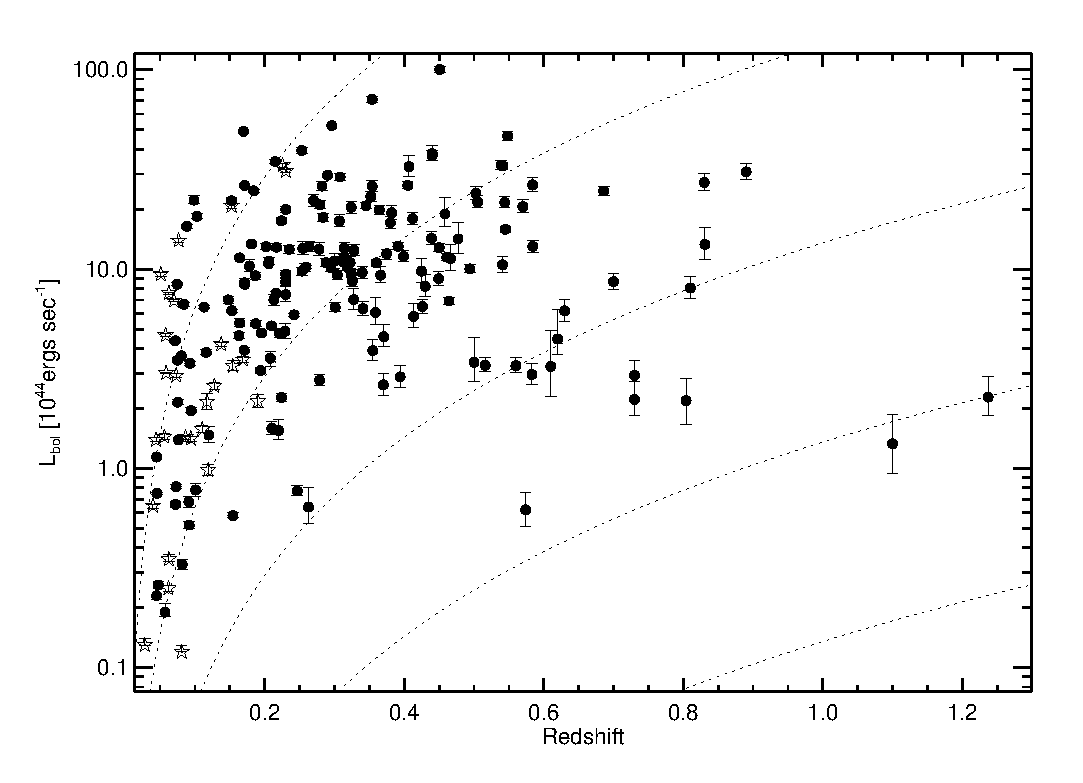
\includegraphics[scale=1.0]{lx_z}
\caption{\small Luminosity plotted as a function of redshift for the
sample. Dotted lines represent constant fluxes of $3.0\times10^{-14},
3.0\times10^{-13}$, and $3.0\times10^{-12} ergs$ $sec^{-1}$ $cm^{-2}$.}
\label{fig:lx_z}
\end{center}
\end{figure}

\begin{figure}[htp]
\begin{center}
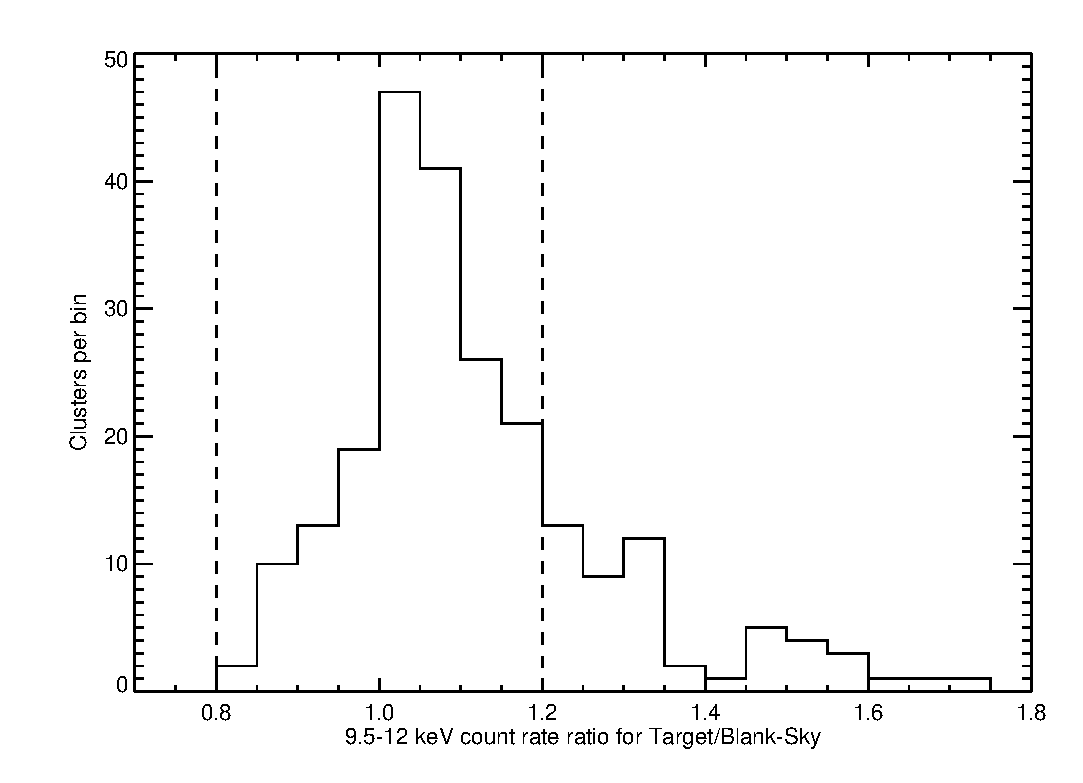
\includegraphics[scale=1.0]{bgd_fig}
\caption{\small Ratio of observation and blank-sky background
count rates in the [9.5-12.0]keV band for each cluster in the sample.}
\label{fig:bgd}
\end{center}
\end{figure}

\begin{figure}[htp]
\begin{center}
\includegraphics[scale=1.0]{rass}
\caption{\small Galactic coordinates of the centroid for each cluster
observation (red circles) overlaid on the {\textit{ROSAT}} All-Sky Survey $3/4$keV
X-Ray background map.}
\label{fig:rass}
\end{center}
\end{figure}

\begin{figure}[htp]
\begin{center}
\includegraphics[scale=1.0]{tx_tx}
\caption{\small Best-fit spectral temperatures for $kT_{S,[0.7-7.0]}$
versus $kT_{S,[2.0-7.0]}$. The line of equality is shown as a dashed,
black line while the best-fit power-law is a solid, red line. Errors
are 90\% confidence (1.6$\sigma$). Linear correlation coefficients are
listed for each fit in lieu of $\chi^2$ values. The mean scatter about
the best-fit line is $\approx5\%$ for all apertures.}
\label{fig:tx_tx}
\end{center}
\end{figure}

\begin{figure}[htp]
\begin{center}
\includegraphics[scale=0.75,angle=-90]{specex}
\caption{\small temporary}
\label{fig:specex}
\end{center}
\end{figure}

\begin{figure}[htp]
\begin{center}
\includegraphics[scale=1.0]{dtx_tx}
\caption{\small Fractional difference between $kT_{S,[0.7-7.0]}$ and
$kT_{S,[2.0-7.0]}$ spectral temperatures versus
$kT_{S,[2.0-7.0]}$. The best-fit linear regression is the solid, red line. Errors
are propogated from the 90\% confidence (1.6$\sigma$) errors of the
best-fit T$_Spec$. Linear correlation coefficients are
listed for each fit in lieu of $\chi^2$ values.}
\label{fig:dtx_tx}
\end{center}
\end{figure}

\begin{figure}[htp]
\begin{center}
\includegraphics[scale=1.0]{plaw_fig}
\caption{\small Best-fit power laws of the form $kT_{S,[0.7-7.0]} =
\alpha kT_{S,[2.0/(1+z)-7.0]}^{\beta}$ to best-fit temperatures for
apertures of varying size.}
\label{fig:plaws}
\end{center}
\end{figure}

\begin{figure}[htp]
\begin{center}
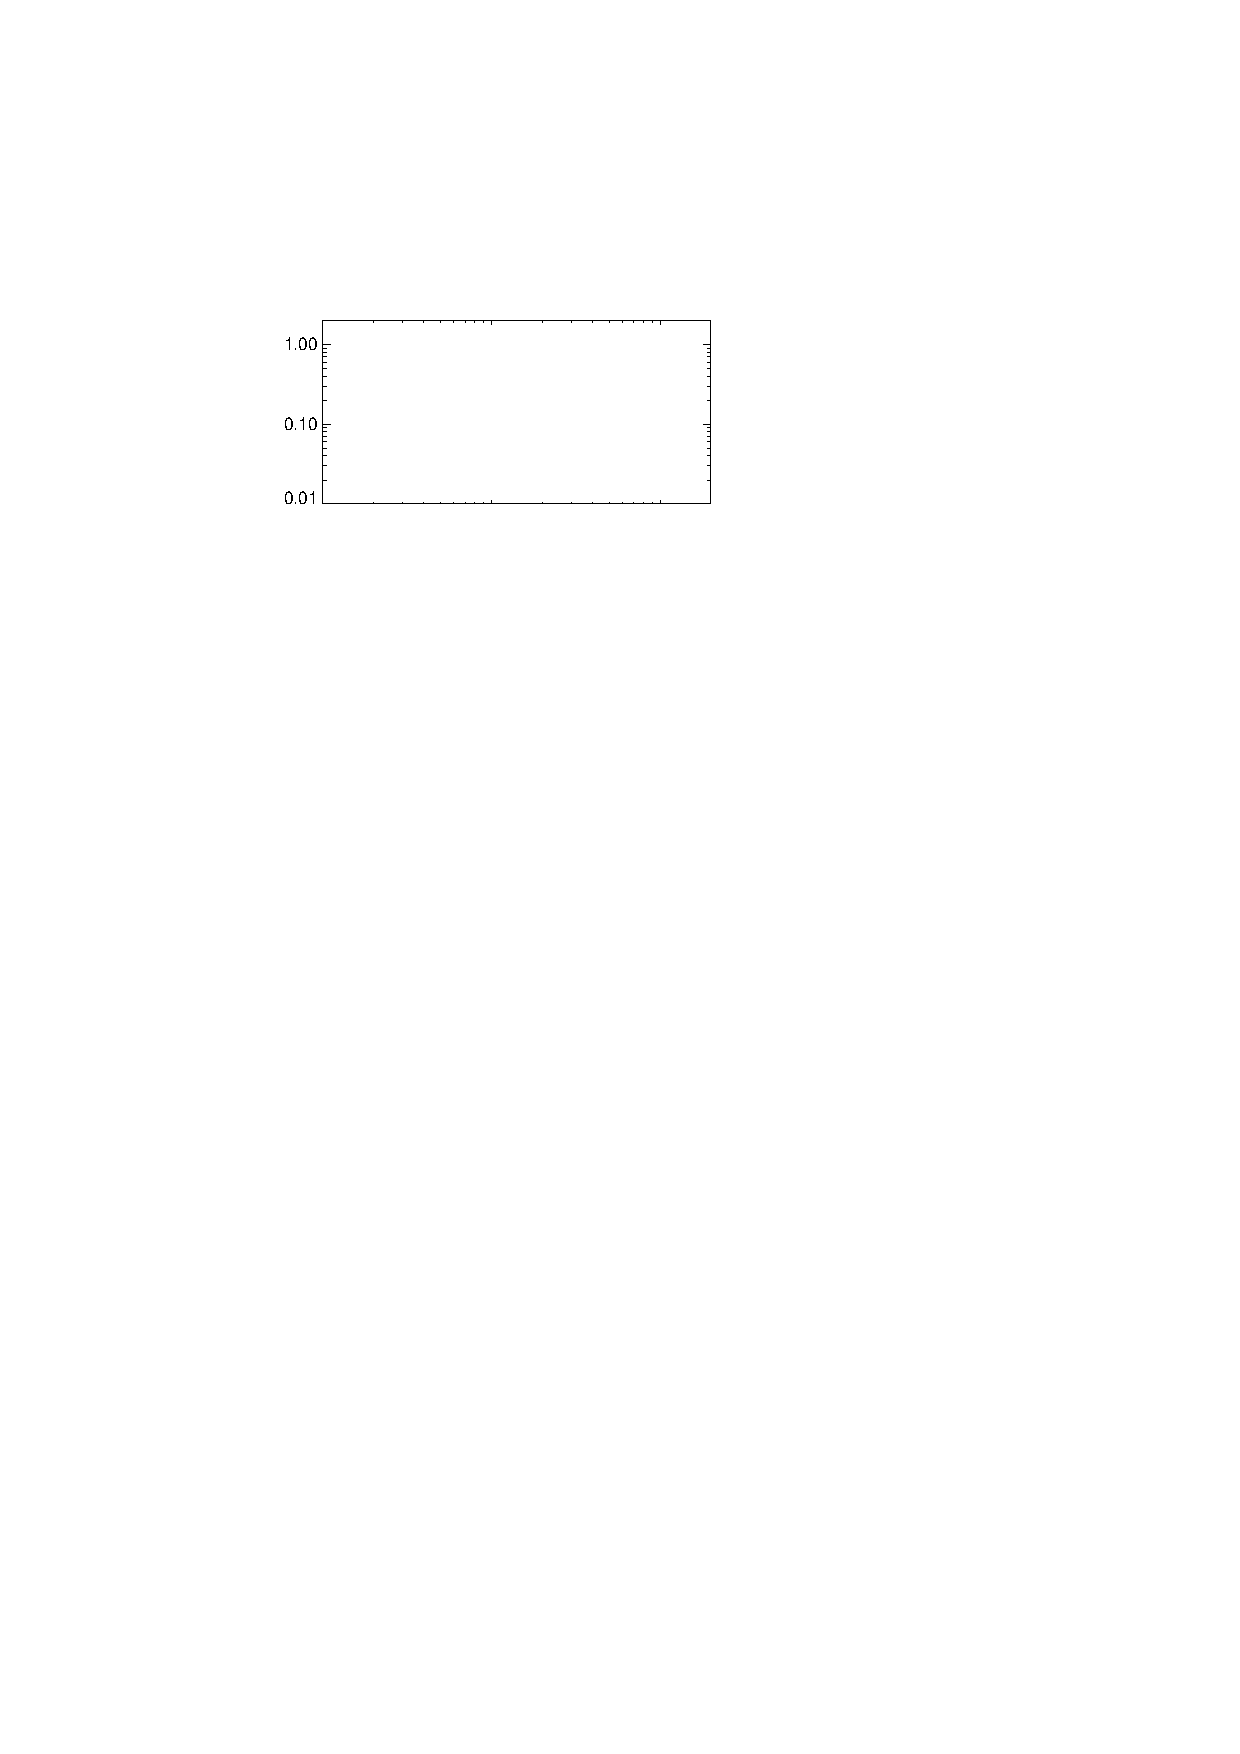
\includegraphics[scale=1.0]{fe_z}
\caption{\small Best-fit metallicity plotted against redshift for our
entire sample.} 
\label{fig:fe_z}
\end{center}
\end{figure}

\begin{figure}[htp]
\begin{center}
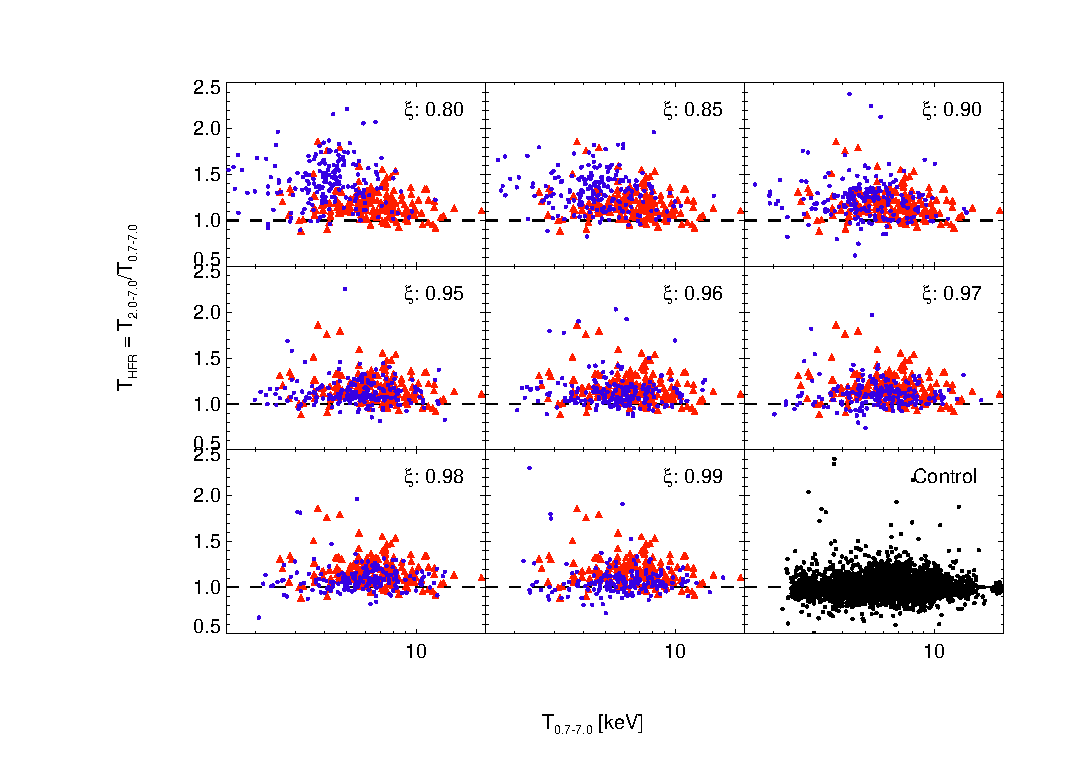
\includegraphics[scale=1.0]{fak_tx}
\caption{\small Best-fit spectral temperatures to simulated spectra
for $kT_{S,[0.7-7.0]}$
versus $kT_{S,[2.0-7.0]}$. The line of equality is shown as a dashed,
black line while the best-fit power-law is a solid line. Errors
are 90\% confidence (1.6$\sigma$).}
\label{fig:fak_tx}
\end{center}
\end{figure}

%%%%%%%%%%
% Tables %
%%%%%%%%%%

\begin{landscape}
\begin{deluxetable}{lcrrccccccccccc}
\tablewidth{0pt}
\tabletypesize{\scriptsize}
\tablecaption{Summary of Sample\label{tab:sample}}
\tablehead{\colhead{Cluster} & \colhead{Obs.ID} & \colhead{R.A.} &
\colhead{Dec.} & \colhead{ExpT} & \colhead{Mode} & \colhead{z} &
\colhead{N$_{H}$} & \colhead{$k$T$_{X}$} & \colhead{Z} &
\colhead{ACIS} & \colhead{L$_{X}$ $10^{44}$} & \colhead{$_{obs}$} & \colhead{$R_{max}$} & \colhead{$R_{break}$}\\
\colhead{ } & \colhead{ } & \colhead{hr:min:sec} & \colhead{$\degr:\arcmin:\arcsec$} & \colhead{ksec} & \colhead{ } & \colhead{ } & \colhead{$10^{20} cm^{-2}$} & \colhead{keV} & \colhead{Z$_{\sun}$} & \colhead{ } & \colhead{$h_{70}^{-2}$ ergs s$^{-1}$} & \colhead{keV} & \colhead{pix} & \colhead{pix}\\
\colhead{{(1)}} & \colhead{{(2)}} & \colhead{{(3)}} & \colhead{{(4)}} & \colhead{{(5)}} & \colhead{{(6)}} & \colhead{{(7)}} & \colhead{{(8)}} & \colhead{{(9)}} & \colhead{{(10)}} & \colhead{{(11)}} & \colhead{{(12)}} & \colhead{{(13)}} & \colhead{{(14)}} & \colhead{{(15)}}
}
\startdata
1RXS J2129.4-0741 & 3595 & 21:29:26.016 & -07:41:29.36 & 19.9 & VF & 0.5700 & 4.36 & 8.62 & 0.52 & I3 & 19.49 & 1.27 & 300 & 110\\
3C 220.1 &  839 & 09:32:40.218 & +79:06:29.46 & 18.9 &  F & 0.6100 & 1.91 & 6.80 & 0.30 & S3 &  3.99 & 1.24 & 200 &  58\\
3C 28.0 & 3233 & 00:55:50.401 & +26:24:36.47 & 49.7 & VF & 0.1952 & 5.71 & 3.90 & 0.12 & I3 & 11.15 & 1.67 & 835 & 739\\
3C 295 & 2254 & 14:11:20.280 & +52:12:10.55 & 90.9 & VF & 0.4641 & 1.35 & 6.51 & 0.36 & I3 &  5.46 & 1.37 & 900 & 153\\
3C 295 &  578 & 14:11:20.486 & +52:12:12.47 & 18.8 &  F & 0.4641 & 1.35 & 6.51 & 0.36 & S3 &  0.00 & 1.37 & 232 & 128\\
4C 55.16 & 4940 & 08:34:54.923 & +55:34:21.15 & 96.0 & VF & 0.2420 & 4.00 & 4.21 & 0.29 & S3 &  4.97 & 1.61 & 360 & 240\\
ABELL 0068 & 3250 & 00:37:06.309 & +09:09:32.28 & 10.0 & VF & 0.2546 & 4.60 & 10.00 & 0.30 & I3 & 10.19 & 1.59 & 590 & 250\\
ABELL 0133 & 2203 & 01:02:41.756 & -21:52:49.79 & 35.5 &  F & 0.0558 & 1.56 & 3.71 & 0.64 & S3 &  0.61 & 1.89 & 313 & 312\\
ABELL 0267 & 3580 & 01:52:42.170 & +01:00:45.63 & 19.9 & VF & 0.2300 & 2.74 & 6.79 & 0.26 & I3 &  8.93 & 1.63 & 590 & 202\\
ABELL 0370 &  515 & 02:39:53.169 & -01:34:36.96 & 88.0 &  F & 0.3747 & 3.37 & 7.20 & 0.39 & S3 & 13.72 & 1.45 & 315 & 315\\
ABELL 0383 & 2321 & 02:48:03.364 & -03:31:44.69 & 19.5 &  F & 0.1871 & 4.07 & 3.93 & 0.38 & S3 &  4.42 & 1.68 & 359 & 266\\
ABELL 0399 & 3230 & 02:57:54.931 & +13:01:58.41 & 48.6 & VF & 0.0716 & 11.51 & 5.80 & 0.23 & I0 &  3.96 & 1.87 & 1016 & 812\\
ABELL 0478 & 1669 & 04:13:25.345 & +10:27:55.64 & 42.4 &  F & 0.0883 & 30.90 & 7.07 & 0.31 & S3 & 10.24 & 1.84 & 414 & 412\\
ABELL 0478 & 6102 & 04:13:25.214 & +10:27:55.13 & 10.0 & VF & 0.0883 & 30.90 & 7.07 & 0.31 & I3 & 12.27 & 1.84 & 812 & 422\\
ABELL 0496 & 3361 & 04:33:37.802 & -13:15:40.14 & 10.0 & VF & 0.0328 & 4.57 & 3.89 & 0.47 & S3 &  0.28 & 1.94 & 300 & 300\\
ABELL 0520 & 4215 & 04:54:09.711 & +02:55:23.69 & 66.3 & VF & 0.2020 & 7.84 & 7.40 & 0.25 & I3 & 10.53 & 1.66 & 468 & 448\\
ABELL 0521 &  430 & 04:54:07.004 & -10:13:26.72 & 39.1 & VF & 0.2533 & 6.17 & 6.74 & 0.19 & S3 & 11.05 & 1.60 & 462 & 462\\
ABELL 0576 & 3289 & 07:21:30.394 & +55:45:41.95 & 38.6 & VF & 0.0385 & 5.57 & 4.09 & 0.46 & S3 &  0.38 & 1.93 & 477 & 477\\
ABELL 0586 &  530 & 07:32:20.339 & +31:37:58.59 & 10.0 & VF & 0.1710 & 5.40 & 8.70 & 0.30 & I3 &  7.50 & 1.71 & 590 & 188\\
ABELL 0611 & 3194 & 08:00:56.832 & +36:03:24.09 & 36.1 & VF & 0.2880 & 4.99 & 6.69 & 0.19 & S3 &  9.03 & 1.55 & 361 & 183\\
ABELL 0644 & 2211 & 08:17:25.225 & -07:30:40.03 & 29.7 & VF & 0.0698 & 6.31 & 6.60 & 0.29 & I3 &  5.26 & 1.87 & 778 & 708\\
ABELL 0665 & 3586 & 08:30:59.231 & +65:50:37.78 & 29.7 & VF & 0.1810 & 4.24 & 8.30 & 0.19 & I3 & 12.61 & 1.69 & 577 & 410\\
ABELL 0697 & 4217 & 08:42:57.549 & +36:21:57.65 & 19.5 & VF & 0.2820 & 3.34 & 9.06 & 0.23 & I3 & 23.61 & 1.56 & 600 & 254\\
ABELL 0773 & 5006 & 09:17:52.566 & +51:43:38.18 & 19.8 & VF & 0.2170 & 1.46 & 8.53 & 0.34 & I3 & 11.44 & 1.64 & 607 & 254\\
ABELL 0781 &  534 & 09:20:25.431 & +30:30:07.56 & 9.9 & VF & 0.2984 & 1.90 & 10.80 & 0.30 & I3 &  9.00 & 1.54 & 560 & 244\\
ABELL 0907 & 3185 & 09:58:21.880 & -11:03:52.20 & 48.0 & VF & 0.1527 & 5.69 & 5.04 & 0.25 & I3 &  5.94 & 1.74 & 702 & 370\\
ABELL 0963 &  903 & 10:17:03.744 & +39:02:49.17 & 36.3 &  F & 0.2056 & 1.39 & 6.60 & 0.34 & S3 &  8.46 & 1.66 & 371 & 371\\
ABELL 1060 & 2220 & 10:36:42.828 & -27:31:42.06 & 31.9 & VF & 0.0125 & 4.96 & 3.20 & 0.37 & I3 &  0.00 & 1.98 & 446 & 444\\
ABELL 1068 & 1652 & 10:40:44.520 & +39:57:10.28 & 26.8 &  F & 0.1375 & 0.71 & 3.87 & 0.42 & S3 &  3.66 & 1.76 & 375 & 266\\
ABELL 1204 & 2205 & 11:13:20.419 & +17:35:38.45 & 23.6 & VF & 0.1706 & 1.44 & 3.78 & 0.35 & I3 &  3.56 & 1.71 & 682 & 202\\
ABELL 1361 & 2200 & 11:43:39.827 & +46:21:21.40 & 16.7 &  F & 0.1171 & 2.18 & 4.08 & 0.61 & S3 &  2.08 & 1.79 & 358 & 162\\
ABELL 1413 & 5003 & 11:55:17.893 & +23:24:21.84 & 75.1 & VF & 0.1426 & 2.19 & 8.90 & 0.21 & I2 &  7.62 & 1.75 & 340 & 335\\
ABELL 1423 &  538 & 11:57:17.026 & +33:36:37.44 & 9.8 & VF & 0.2130 & 1.60 & 8.50 & 0.30 & I3 &  6.77 & 1.65 & 520 & 136\\
ABELL 1650 & 4178 & 12:58:41.499 & -01:45:44.32 & 27.3 & VF & 0.0843 & 1.62 & 5.89 & 0.40 & S3 &  3.26 & 1.84 & 358 & 354\\
ABELL 1651 & 4185 & 12:59:22.830 & -04:11:45.86 & 9.6 & VF & 0.0840 & 2.02 & 7.00 & 0.32 & I3 &  5.69 & 1.84 & 888 & 370\\
ABELL 1664 & 1648 & 13:03:42.478 & -24:14:44.55 & 9.8 & VF & 0.1276 & 8.47 & 3.50 & 0.11 & S3 &  2.52 & 1.77 & 358 & 176\\
ABELL 1682 & 3244 & 13:06:50.764 & +46:33:19.86 & 9.8 & VF & 0.2260 & 1.10 & 8.90 & 0.30 & I3 &  7.28 & 1.63 & 460 & 313\\
ABELL 1689 & 5004 & 13:11:29.474 & -01:20:25.17 & 19.9 & VF & 0.1843 & 1.87 & 10.10 & 0.25 & I3 & 20.22 & 1.69 & 607 & 332\\
ABELL 1758 & 2213 & 13:32:42.978 & +50:32:44.83 & 58.3 & VF & 0.2792 & 1.09 & 7.95 & 0.20 & S3 & 206.59 & 1.56 & 461 & 344\\
ABELL 1763 & 3591 & 13:35:17.957 & +40:59:55.80 & 19.6 & VF & 0.1866 & 0.82 & 6.90 & 0.16 & I3 &  8.99 & 1.69 & 647 & 471\\
ABELL 1835 &  495 & 14:01:01.951 & +02:52:43.18 & 19.5 &  F & 0.2532 & 2.36 & 7.65 & 0.36 & S3 & 27.75 & 1.60 & 384 & 384\\
ABELL 1942 & 3290 & 14:38:21.878 & +03:40:12.97 & 57.6 & VF & 0.2240 & 2.75 & 5.12 & 0.27 & I2 &  3.44 & 1.63 & 633 & 214\\
ABELL 1991 & 3193 & 14:54:31.620 & +18:38:41.48 & 38.3 & VF & 0.0565 & 2.43 & 5.40 & 0.30 & S3 &  0.33 & 1.89 & 370 & 370\\
ABELL 2029 & 4977 & 15:10:56.139 & +05:44:40.96 & 77.9 &  F & 0.0765 & 3.26 & 7.38 & 0.42 & S3 &  7.89 & 1.86 & 366 & 363\\
ABELL 2029 & 6101 & 15:10:56.064 & +05:44:40.40 & 9.9 & VF & 0.0765 & 3.26 & 7.38 & 0.42 & I3 & 11.13 & 1.86 & 815 & 500\\
ABELL 2034 & 2204 & 15:10:11.003 & +33:30:46.46 & 53.9 & VF & 0.1130 & 1.58 & 7.15 & 0.29 & I3 &  6.34 & 1.80 & 920 & 604\\
ABELL 2104 &  895 & 15:40:08.591 & -03:18:07.14 & 49.2 &  F & 0.1554 & 14.93 & 9.31 & 0.32 & S3 &  4.98 & 1.73 & 299 & 294\\
ABELL 2111 &  544 & 15:39:41.432 & +34:25:12.26 & 10.3 &  F & 0.2300 & 2.20 & 8.02 & 0.30 & I3 &  8.02 & 1.63 & 605 & 338\\
ABELL 2124 & 3238 & 15:44:59.131 & +36:06:34.11 & 19.4 & VF & 0.0658 & 1.71 & 2.50 & 0.30 & S3 &  0.37 & 1.88 & 338 & 176\\
ABELL 2142 & 1228 & 15:58:19.884 & +27:13:46.08 & 12.1 &  F & 0.0898 & 4.31 & 8.24 & 0.28 & S3 &  0.00 & 1.84 & 262 & 262\\
ABELL 2147 & 3211 & 16:02:13.476 & +15:57:58.32 & 17.9 & VF & 0.0356 & 3.38 & 4.45 & 0.35 & I1 &  0.66 & 1.93 & 947 & 681\\
ABELL 2163 & 1653 & 16:15:45.705 & -06:09:00.62 & 71.1 & VF & 0.1695 & 12.04 & 12.12 & 0.22 & I1 & 28.62 & 1.71 & 767 & 767\\
ABELL 2199 &  497 & 16:28:38.249 & +39:33:04.28 & 19.5 &  F & 0.0300 & 0.88 & 4.14 & 0.43 & S3 &  0.43 & 1.94 & 353 & 352\\
ABELL 2204 &  499 & 16:32:46.986 & +05:34:30.89 & 10.1 &  F & 0.1524 & 5.84 & 6.97 & 0.38 & S3 & 15.28 & 1.74 & 377 & 377\\
ABELL 2204 & 6104 & 16:32:46.944 & +05:34:31.22 & 9.6 & VF & 0.1524 & 5.84 & 9.00 & 0.30 & I3 & 17.68 & 1.74 & 827 & 280\\
ABELL 2218 & 1666 & 16:35:50.831 & +66:12:42.31 & 48.6 & VF & 0.1713 & 3.12 & 6.70 & 0.30 & I0 &  8.72 & 1.71 & 783 & 396\\
ABELL 2219 &  896 & 16:40:21.069 & +46:42:29.07 & 42.3 &  F & 0.2256 & 1.76 & 9.81 & 0.27 & S3 & 24.66 & 1.63 & 365 & 362\\
ABELL 2244 & 4179 & 17:02:42.579 & +34:03:37.34 & 57.0 & VF & 0.0967 & 2.09 & 5.57 & 0.29 & S3 &  4.24 & 1.82 & 361 & 360\\
ABELL 2255 &  894 & 17:12:40.385 & +64:03:50.63 & 39.4 &  F & 0.0805 & 2.53 & 6.42 & 0.25 & I3 &  3.85 & 1.85 & 970 & 855\\
ABELL 2259 & 3245 & 17:20:08.299 & +27:40:11.53 & 10.0 & VF & 0.1640 & 3.70 & 4.94 & 0.30 & I3 &  5.47 & 1.72 & 585 & 348\\
ABELL 2261 & 5007 & 17:22:27.254 & +32:07:58.60 & 24.3 & VF & 0.2240 & 3.31 & 7.58 & 0.30 & I3 & 15.61 & 1.63 & 591 & 266\\
ABELL 2294 & 3246 & 17:24:10.149 & +85:53:09.77 & 10.0 & VF & 0.1780 & 6.10 & 7.10 & 0.30 & I3 &  8.19 & 1.70 & 620 & 276\\
ABELL 2319 & 3231 & 19:21:12.280 & +43:55:57.89 & 14.4 & VF & 0.0562 & 9.05 & 9.49 & 0.25 & I1 &  8.18 & 1.89 & 947 & 904\\
ABELL 2384 & 4202 & 21:52:21.178 & -19:32:51.90 & 31.5 & VF & 0.0945 & 2.99 & 3.80 & 0.30 & I3 &  2.48 & 1.83 & 760 & 344\\
ABELL 2390 & 4193 & 21:53:36.825 & +17:41:44.38 & 95.1 & VF & 0.2301 & 6.71 & 9.16 & 0.25 & S3 & 22.35 & 1.63 & 350 & 345\\
ABELL 2409 & 3247 & 22:00:52.567 & +20:58:34.11 & 10.2 & VF & 0.1479 & 6.72 & 5.50 & 0.30 & I3 &  6.14 & 1.74 & 470 & 300\\
ABELL 2537 & 4962 & 23:08:22.313 & -02:11:29.88 & 36.2 & VF & 0.2950 & 4.26 & 6.08 & 0.26 & S3 &  7.76 & 1.54 & 362 & 174\\
ABELL 2550 & 2225 & 23:11:35.806 & -21:44:46.70 & 59.0 & VF & 0.1543 & 2.03 & 2.58 & 0.30 & S3 &  0.64 & 1.73 & 480 & 188\\
ABELL 2554 & 1696 & 23:12:19.939 & -21:30:09.84 & 19.9 & VF & 0.1103 & 2.04 & 6.40 & 0.44 & S3 &  1.42 & 1.80 & 450 & 391\\
ABELL 2556 & 2226 & 23:13:01.413 & -21:38:04.47 & 19.9 & VF & 0.0862 & 2.02 & 4.13 & 0.34 & S3 &  1.26 & 1.84 & 475 & 280\\
ABELL 2589 & 3210 & 23:23:57.315 & +16:46:38.43 & 13.7 & VF & 0.0415 & 3.98 & 3.70 & 0.30 & S3 &  0.21 & 1.92 & 290 & 276\\
ABELL 2597 &  922 & 23:25:19.779 & -12:07:27.63 & 39.4 &  F & 0.0854 & 2.51 & 3.58 & 0.37 & S3 &  0.73 & 1.84 & 138 & 134\\
ABELL 2626 & 3192 & 23:36:30.452 & +21:08:47.36 & 24.8 & VF & 0.0573 & 4.30 & 2.90 & 0.30 & S3 &  0.48 & 1.89 & 378 & 358\\
ABELL 2667 & 2214 & 23:51:39.395 & -26:05:02.75 & 9.6 & VF & 0.2300 & 1.64 & 6.31 & 0.31 & S3 & 16.05 & 1.63 & 367 & 188\\
ABELL 2670 & 4959 & 23:54:13.687 & -10:25:08.85 & 39.6 & VF & 0.0763 & 2.88 & 3.98 & 0.25 & I3 &  1.34 & 1.86 & 883 & 410\\
ABELL 2744 & 2212 & 00:14:14.396 & -30:22:40.04 & 24.8 & VF & 0.3080 & 1.82 & 9.61 & 0.19 & S3 & 26.35 & 1.53 & 460 & 453\\
ABELL 3112 & 2516 & 03:17:57.681 & -44:14:17.16 & 16.9 & VF & 0.0720 & 2.50 & 4.28 & 0.51 & S3 &  2.52 & 1.87 & 366 & 366\\
ABELL 3158 & 3201 & 03:42:54.675 & -53:37:24.36 & 24.8 & VF & 0.0580 & 1.60 & 5.50 & 0.30 & I3 &  2.96 & 1.89 & 863 & 760\\
ABELL 3266 &  899 & 04:31:14.960 & -61:27:32.23 & 29.8 & VF & 0.0590 & 1.72 & 8.35 & 0.32 & I1 &  1.99 & 1.89 & 463 & 462\\
ABELL 3558 & 1646 & 13:27:56.854 & -31:29:43.78 & 14.4 & VF & 0.0480 & 3.84 & 5.51 & 0.33 & S3 &  1.14 & 1.91 & 370 & 365\\
ABELL 3562 & 4167 & 13:33:36.566 & -31:40:27.78 & 19.3 & VF & 0.0490 & 3.90 & 3.80 & 0.30 & I2 &  0.95 & 1.91 & 660 & 448\\
ABELL 3571 & 4203 & 13:47:28.434 & -32:51:52.45 & 34.0 & VF & 0.0391 & 4.66 & 7.60 & 0.30 & S3 &  0.60 & 1.92 & 265 & 262\\
ABELL 3667 & 5751 & 20:12:41.231 & -56:50:35.70 & 128.9 & VF & 0.0556 & 5.45 & 6.72 & 0.29 & I3 &  3.44 & 1.89 & 745 & 744\\
ABELL 4038 & 4992 & 23:47:44.668 & -28:08:19.07 & 33.5 & VF & 0.0300 & 1.57 & 3.30 & 0.30 & I2 &  0.64 & 1.94 & 976 & 864\\
AC 114 & 1562 & 22:58:48.196 & -34:47:56.89 & 72.5 &  F & 0.3120 & 1.44 & 6.99 & 0.30 & S3 & 12.50 & 1.52 & 442 & 441\\
CL 0024+17 &  929 & 00:26:35.996 & +17:09:45.37 & 39.8 &  F & 0.3940 & 4.36 & 4.80 & 0.30 & S3 &  4.67 & 1.43 & 393 & 114\\
CL 1221+4918 & 1662 & 12:21:26.709 & +49:18:21.60 & 79.1 & VF & 0.7000 & 1.44 & 7.20 & 0.30 & I3 &  7.99 & 1.18 & 584 & 110\\
CL J0542.8-4100 &  914 & 05:42:49.994 & -40:59:58.50 & 50.4 &  F & 0.6300 & 3.59 & 6.62 & 0.30 & I3 &  7.68 & 1.23 & 840 &  84\\
CL J1113.1-2615 &  915 & 11:13:05.167 & -26:15:40.43 & 104.6 &  F & 0.7300 & 5.51 & 7.14 & 0.30 & I3 &  3.41 & 1.16 & 735 &  58\\
CL J1226.9+3332 &  932 & 12:26:58.157 & +33:32:49.57 & 9.8 & VF & 0.8900 & 1.37 & 10.00 & 0.30 & S3 & 19.26 & 1.06 & 280 &  84\\
CL J2302.8+0844 &  918 & 23:02:48.156 & +08:43:52.74 & 108.6 &  F & 0.7300 & 5.05 & 10.00 & 0.30 & I3 &  3.65 & 1.16 & 830 &  84\\
CYGNUS A &  360 & 19:59:28.381 & +40:44:01.98 & 34.7 &  F & 0.0561 & 35.23 & 10.40 & 0.72 & S3 &  1.23 & 1.89 & 292 & 291\\
ESO 3060170 & 3189 & 05:40:06.679 & -40:50:11.97 & 14.1 & VF & 0.0358 & 3.43 & 2.63 & 0.30 & I0 &  0.20 & 1.93 & 645 & 280\\
ESO 5520200 & 3206 & 04:54:52.318 & -18:06:56.52 & 23.9 & VF & 0.0314 & 4.29 & 2.34 & 0.30 & I3 &  0.08 & 1.94 & 704 & 176\\
EXO 0422-086 & 4183 & 04:25:51.271 & -08:33:36.42 & 10.0 & VF & 0.0397 & 6.22 & 3.28 & 0.30 & I3 &  0.58 & 1.92 & 960 & 318\\
HERCULES A & 1625 & 16:51:08.161 & +04:59:32.44 & 14.8 & VF & 0.1541 & 6.27 & 4.15 & 0.45 & S3 &  2.79 & 1.73 & 283 & 188\\
IRAS 09104+4109 &  509 & 09:13:45.481 & +40:56:27.49 & 9.1 &  F & 0.4420 & 1.36 & 8.98 & 0.30 & S3 & 52.89 & 1.39 & 328 & 110\\
M87 &  352 & 12:30:49.411 & +12:23:28.13 & 37.7 & GRADED & 0.0043 & 2.55 & 2.40 & 0.30 & S3 &  0.00 & 1.99 & 295 & 294\\
MACS J0011.7-1523 & 6105 & 00:11:42.957 & -15:23:20.46 & 37.3 & VF & 0.3600 & 2.08 & 5.42 & 0.30 & I3 &  9.52 & 1.47 & 757 & 179\\
MACS J0159.8-0849 & 6106 & 01:59:49.422 & -08:50:00.42 & 35.3 & VF & 0.4050 & 2.01 & 9.59 & 0.30 & I3 & 20.64 & 1.42 & 737 & 166\\
MACS J0242.5-2132 & 3266 & 02:42:35.906 & -21:32:26.30 & 11.9 & VF & 0.3140 & 2.71 & 6.22 & 0.20 & I3 & 11.89 & 1.52 & 683 & 112\\
MACS J0329.6-0211 & 3582 & 03:29:41.622 & -02:11:46.82 & 19.9 & VF & 0.4500 & 6.21 & 5.24 & 0.30 & I3 & 12.81 & 1.38 & 555 & 127\\
MACS J0429.6-0253 & 3271 & 04:29:36.088 & -02:53:09.02 & 23.2 & VF & 0.3990 & 5.70 & 6.76 & 0.40 & I3 & 10.64 & 1.43 & 676 & 124\\
MACS J0547.0-3904 & 3273 & 05:47:01.582 & -39:04:28.24 & 21.7 & VF & 0.2100 & 4.08 & 2.96 & 0.30 & I3 &  1.91 & 1.65 & 678 & 119\\
MACS J0744.9+3927 & 6111 & 07:44:52.842 & +39:27:26.28 & 49.5 & VF & 0.6860 & 4.66 & 11.29 & 0.30 & I3 & 20.94 & 1.19 & 740 & 143\\
MACS J1115.8+0129 & 3275 & 11:15:52.048 & +01:29:56.56 & 15.9 & VF & 0.1200 & 4.36 & 4.10 & 0.30 & I3 &  1.21 & 1.79 & 650 & 146\\
MACS J1311.0-0311 & 6110 & 13:11:01.647 & -03:10:37.78 & 63.2 & VF & 0.4940 & 2.18 & 6.70 & 0.30 & I3 &  7.55 & 1.34 & 753 & 153\\
MACS J1427.6-2521 & 3279 & 14:27:39.389 & -25:21:04.66 & 16.9 & VF & 0.2200 & 6.11 & 3.80 & 0.40 & I3 &  1.93 & 1.64 & 666 & 104\\
MACS J1621.3+3810 & 3594 & 16:21:24.933 & +38:10:06.57 & 19.7 & VF & 0.4610 & 1.07 & 7.53 & 0.30 & I3 & 11.22 & 1.37 & 572 & 124\\
MACS J1621.6+3810 & 6109 & 16:21:24.742 & +38:10:08.92 & 37.5 & VF & 0.4610 & 1.07 & 7.53 & 0.30 & I3 &  9.44 & 1.37 & 756 & 123\\
MACS J1931.8-2634 & 3282 & 19:31:49.656 & -26:34:33.99 & 13.6 & VF & 0.3520 & 9.13 & 7.50 & 0.20 & I3 & 20.79 & 1.48 & 670 & 148\\
MACS J2229.7-2755 & 3286 & 22:29:45.358 & -27:55:38.41 & 16.4 & VF & 0.3240 & 1.34 & 5.50 & 0.30 & I3 &  8.71 & 1.51 & 684 & 117\\
MKW 04 & 3234 & 12:04:27.218 & +01:53:42.79 & 30.0 & VF & 0.0198 & 1.90 & 2.16 & 0.43 & S3 &  0.02 & 1.96 & 467 & 343\\
MS 0016.9+1609 &  520 & 00:18:33.503 & +16:26:12.99 & 67.4 & VF & 0.5410 & 4.06 & 9.90 & 0.30 & I3 & 31.42 & 1.30 & 608 & 240\\
MS 0302.7+1658 &  525 & 03:05:31.614 & +17:10:02.06 & 10.0 & VF & 0.4240 & 10.95 & 3.60 & 0.30 & I3 &  2.96 & 1.40 & 569 &  75\\
MS 0440.5+0204 & 4196 & 04:43:09.952 & +02:10:18.70 & 59.4 & VF & 0.1900 & 9.10 & 10.00 & 0.30 & S3 &  5.91 & 1.68 & 368 &  84\\
MS 0451.6-0305 &  902 & 04:54:11.004 & -03:00:52.19 & 44.2 &  F & 0.5386 & 5.68 & 8.62 & 0.28 & S3 & 26.46 & 1.30 & 460 & 254\\
MS 0735.6+7421 & 4197 & 07:41:44.245 & +74:14:38.23 & 45.5 & VF & 0.2160 & 3.40 & 5.45 & 0.37 & S3 &  6.58 & 1.64 & 343 & 280\\
MS 0839.8+2938 & 2224 & 08:42:55.969 & +29:27:26.97 & 29.8 &  F & 0.1940 & 3.92 & 3.80 & 0.59 & S3 &  3.07 & 1.68 & 374 & 176\\
MS 0906.5+1110 &  924 & 09:09:12.753 & +10:58:32.00 & 29.7 & VF & 0.1630 & 3.60 & 8.10 & 0.30 & I3 &  4.47 & 1.72 & 585 & 254\\
MS 1006.0+1202 &  925 & 10:08:47.194 & +11:47:55.99 & 29.4 & VF & 0.2210 & 3.63 & 7.03 & 0.37 & I3 &  5.15 & 1.64 & 572 & 188\\
MS 1008.1-1224 &  926 & 10:10:32.312 & -12:39:56.80 & 44.2 & VF & 0.3010 & 6.71 & 7.47 & 0.72 & I3 &  8.08 & 1.54 & 569 & 214\\
MS 1054.5-0321 &  512 & 10:56:58.499 & -03:37:32.76 & 89.1 &  F & 0.8300 & 3.69 & 13.21 & 0.07 & S3 & 21.28 & 1.09 & 438 & 214\\
MS 1455.0+2232 & 4192 & 14:57:15.088 & +22:20:32.49 & 91.9 & VF & 0.2590 & 3.35 & 4.51 & 0.35 & I3 &  9.60 & 1.59 & 575 & 318\\
MS 1621.5+2640 &  546 & 16:23:35.522 & +26:34:25.67 & 30.1 &  F & 0.4260 & 3.59 & 7.60 & 0.30 & I3 &  7.91 & 1.40 & 643 & 124\\
MS 2053.7-0449 & 1667 & 20:56:21.295 & -04:37:46.61 & 44.5 & VF & 0.5830 & 5.16 & 10.03 & 0.31 & I3 &  3.11 & 1.26 & 602 &  84\\
MS 2137.3-2353 & 4974 & 21:40:15.178 & -23:39:40.71 & 57.4 & VF & 0.3130 & 3.40 & 6.30 & 0.30 & S3 &  9.10 & 1.52 & 340 & 115\\
OPHIUCHUS & 3200 & 17:12:27.731 & -23:22:06.74 & 50.5 &  F & 0.0280 & 36.00 & 10.00 & 0.30 & S3 &  1.16 & 1.95 & 366 & 363\\
PKS 0745-191 &  508 & 07:47:31.140 & -19:17:38.98 & 28.0 &  F & 0.1028 & 40.82 & 8.50 & 0.30 & S3 & 14.25 & 1.81 & 363 & 362\\
PKS 0745-191 & 6103 & 07:47:31.295 & -19:17:40.50 & 10.3 & VF & 0.1028 & 40.80 & 8.50 & 0.30 & I3 & 12.63 & 1.81 & 806 & 358\\
RBS 0797 & 2202 & 09:47:12.971 & +76:23:13.90 & 11.7 & VF & 0.3540 & 2.22 & 6.43 & 0.30 & I3 & 18.94 & 1.48 & 750 & 136\\
RX J0439+0520 &  527 & 04:39:02.218 & +05:20:43.11 & 9.6 & VF & 0.2080 & 10.02 & 4.63 & 0.30 & I3 &  3.06 & 1.66 & 580 & 103\\
RX J0439.0+0715 & 1449 & 04:39:00.710 & +07:16:08.15 & 6.3 &  F & 0.2400 & 1.10 & 9.50 & 0.30 & I3 & 13.46 & 1.61 & 680 & 124\\
RX J0647.7+7015 & 3584 & 06:47:49.919 & +70:14:54.91 & 20.0 & VF & 0.5840 & 5.18 & 9.07 & 0.30 & I3 & 23.31 & 1.26 & 610 & 110\\
RX J0819.6+6336 & 2199 & 08:19:26.007 & +63:37:26.53 & 14.9 &  F & 0.1190 & 4.11 & 3.90 & 0.30 & S3 &  0.96 & 1.79 & 364 & 188\\
RX J0820.9+0752 & 1647 & 08:21:02.180 & +07:51:48.42 & 9.4 &  F & 0.1100 & 2.37 & 7.28 & 0.30 & S3 &  1.98 & 1.80 & 370 &  84\\
RX J0910+5422 & 2227 & 09:10:44.726 & +54:22:04.46 & 105.7 & VF & 1.1000 & 2.07 & 3.50 & 0.30 & I3 &  2.46 & 0.95 & 624 &  75\\
RX J1347.5-1145 & 3592 & 13:47:30.593 & -11:45:10.05 & 57.7 & VF & 0.4510 & 4.89 & 10.88 & 0.30 & I3 & 59.01 & 1.38 & 708 & 266\\
RX J1347.5-1145 &  507 & 13:47:30.632 & -11:45:09.78 & 10.0 &  F & 0.4510 & 4.89 & 10.88 & 0.37 & S3 & 57.99 & 1.38 & 375 & 214\\
RX J1423.8+2404 & 1657 & 14:23:47.759 & +24:04:40.95 & 18.5 & VF & 0.5450 & 2.65 & 5.92 & 0.30 & I3 & 13.52 & 1.29 & 601 &  98\\
RX J1423.8+2404 & 4195 & 14:23:47.942 & +24:04:43.09 & 115.6 & VF & 0.5450 & 2.65 & 5.92 & 0.30 & S3 & 13.30 & 1.29 & 357 & 188\\
RX J1504.1-0248 & 5793 & 15:04:07.415 & -02:48:15.70 & 39.2 & VF & 0.2150 & 6.27 & 8.90 & 0.30 & I3 & 25.10 & 1.65 & 685 & 320\\
RX J1532.9+3021 & 1649 & 15:32:53.781 & +30:20:58.72 & 9.4 & VF & 0.3450 & 2.21 & 5.44 & 0.34 & S3 & 16.96 & 1.49 & 352 & 124\\
RX J1532.9+3021 & 1665 & 15:32:53.817 & +30:20:58.34 & 10.0 & VF & 0.3450 & 2.21 & 5.44 & 0.30 & I3 & 17.30 & 1.49 & 586 & 136\\
RX J1716.9+6708 &  548 & 17:16:49.015 & +67:08:25.80 & 51.7 &  F & 0.8100 & 3.71 & 9.84 & 0.30 & I3 &  6.23 & 1.10 & 560 &  72\\
RX J1720.1+2638 & 4361 & 17:20:09.941 & +26:37:29.11 & 25.7 & VF & 0.1640 & 4.02 & 5.55 & 0.30 & I3 & 10.15 & 1.72 & 690 & 318\\
RX J1720.2+3536 & 3280 & 17:20:16.792 & +35:36:26.08 & 20.8 & VF & 0.3913 & 3.35 & 5.65 & 0.30 & I3 & 12.81 & 1.44 & 690 & 150\\
RX J2129.6+0005 &  552 & 21:29:39.944 & +00:05:18.83 & 10.0 & VF & 0.2350 & 4.30 & 11.00 & 0.30 & I3 & 11.50 & 1.62 & 610 & 150\\
SERSIC 159-03 & 1668 & 23:13:58.764 & -42:43:34.70 & 9.9 & VF & 0.0580 & 1.89 & 2.41 & 0.30 & S3 &  0.78 & 1.89 & 357 & 306\\
V 1121.0+2327 & 1660 & 11:20:57.195 & +23:26:27.60 & 71.3 & VF & 0.5600 & 1.30 & 6.10 & 0.30 & I3 &  3.56 & 1.28 & 600 & 110\\
ZWCL 1358+6245 &  516 & 13:59:50.526 & +62:31:04.57 & 54.1 &  F & 0.3280 & 1.94 & 7.20 & 0.30 & S3 & 10.81 & 1.51 & 423 & 254\\
ZWCL 1953 & 1659 & 08:50:06.677 & +36:04:16.16 & 24.9 &  F & 0.3800 & 3.10 & 14.50 & 0.30 & I3 & 15.41 & 1.45 & 535 & 150\\
ZWCL 3146 &  909 & 10:23:39.735 & +04:11:08.05 & 46.0 &  F & 0.2900 & 2.70 & 12.80 & 0.30 & I3 & 23.00 & 1.55 & 630 & 292\\
ZWCL 5247 &  539 & 12:34:21.928 & +09:47:02.83 & 9.3 & VF & 0.2290 & 1.70 & 8.50 & 0.30 & I3 &  5.94 & 1.63 & 530 & 435\\
ZWCL 7160 &  543 & 14:57:15.158 & +22:20:33.85 & 9.9 &  F & 0.2578 & 3.10 & 9.60 & 0.30 & I3 &  8.77 & 1.59 & 555 & 124\\
ZWICKY 2701 & 3195 & 09:52:49.183 & +51:53:05.27 & 26.9 & VF & 0.2100 & 0.83 & 4.44 & 0.30 & S3 &  4.42 & 1.65 & 370 & 176\\
\enddata
\tablecomments{name, obsid, Instr, mode, ExpTime, RA, Dec, z, NH, kTx,
Lx is given for the [0.3-10]keV energy band, Fe}
\end{deluxetable}
\end{landscape}

%%%%%%%%%%%%%%%%%%%%%%%%
% Spectral fit results %
%%%%%%%%%%%%%%%%%%%%%%%%

\begin{deluxetable}{lccc}
\tablewidth{0pt}
\tabletypesize{\scriptsize}
\tablecaption{Summary of Spectral Fit Results\label{tab:specfits}}
\tablehead{\colhead{Name} & \colhead{$R_{out}$} & \colhead{$N_H$} & \colhead{$T_X$}\\
\colhead{ } & \colhead{ } & \colhead{ } & \colhead{ }\\
\colhead{{(1)}} & \colhead{{(2)}} & \colhead{{(3)}} & \colhead{{(4)}}
}
\startdata
Is & there & any &  need\\
for &  this & table &  ???\\
\enddata
\tablecomments{
	\begin{enumerate}
	\item Cluster name.
	\item Outer radius as a fraction of r500.
	\item Hydrogen column density in units of $10^{20}$ cm$^{-3}$. 
	\item X-ray temperature in keV and 90\% confidence limits. 
	\end{enumerate}
}
\end{deluxetable}

%%%%%%%%%%%%%%%%%%%%
% End the document %
%%%%%%%%%%%%%%%%%%%%
\end{document}
